\section{هدف تمرین}

در این تمرین یک محاسبه‌گر \lr{CRC-8-ATM} سریال با چندجمله‌ای \lr{P(x) = x\textsuperscript{8} + x\textsuperscript{2} + x + 1} طراحی شده است. داده‌ی ورودی بیت‌به‌بیت و \lr{MSB-first} از طریق \code{in\_data} وارد مدار می‌شود و پس از پردازش \code{length\_msg} بیت، مقدار نهایی روی \code{out\_crc} قرار می‌گیرد و \code{valid} دقیقاً یک سیکل فعال می‌شود.

% =========================================================
\section{توضیح معماری}

مدار از سه ماژول مجزا تشکیل شده که در یک ماژول سطح بالا به نام \code{crc8\_top}
با یکدیگر ترکیب می‌شوند:

\vspace{-0.4cm}

\begin{itemize}
    \item \textbf{\code{d\_ff}}: فلیپ‌فلاپ \lr{D} با ریست آسنکرون \lr{active-low}، \lr{synchronous clear}، و \lr{enable}.
    \item \textbf{\code{crc\_datapath}}: مسیر داده‌ی ساختاری شامل هشت نمونه از \code{d\_ff} و گیت‌های \lr{XOR} برای پیاده‌سازی چندجمله‌ای \lr{CRC-8-ATM}.
    \item \textbf{\code{crc\_controller}}: کنترل‌کننده‌ی رفتاری مبتنی بر \lr{FSM} که با سیگنال‌های \code{en\_shift} و \code{sync\_clr}، مسیر داده را هدایت می‌کند.
\end{itemize}

وقتی \code{sync\_clr = 1} است، تمام فلیپ‌فلاپ‌ها در لبه بالارونده بعدی کلاک
صفر می‌شوند. وقتی \code{en\_shift = 1} است، ثبات \lr{CRC} با محاسبه بیت
جدید بروزرسانی می‌شود. خروجی \code{crc\_out} مستقیماً سیم \code{crc\_value}
از مسیر داده است و هیچ ثبات میانی ندارد.

\subsection{ماشین حالت کنترل‌کننده}

کنترل‌کننده یک \lr{FSM} با چهار حالت است:

\begin{figure}[H]
    \centering
    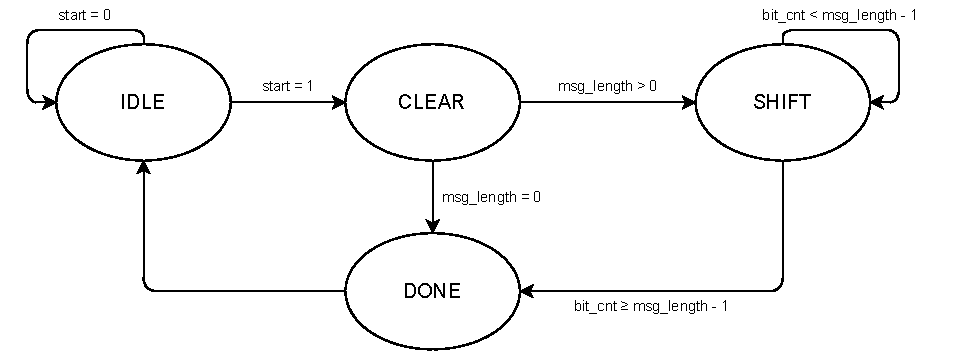
\includegraphics[width=0.70\textwidth]{assets/DSD_HW5_Q4_FSM_diagram.pdf}
    \caption{دیاگرام \lr{FSM} کنترل‌کننده \lr{CRC-8}}
\end{figure}

\begin{LTR}
    \begin{table}[H]
        \centering
        \begin{tabular}{|c|c|c|c|c|c|}
            \hline
            \textbf{فعلی حالت} & \textbf{انتقال شرط}              & \textbf{بعدی حالت}
                               & \textbf{\code{en\_shift}}        & \textbf{\code{sync\_clr}} & \textbf{\code{valid}}         \\
            \hline
            \lr{IDLE}          & \code{start = 0}                 & \lr{IDLE}                 & 0                     & 0 & 0 \\
            \lr{IDLE}          & \code{start = 1}                 & \lr{CLEAR}                & 0                     & 0 & 0 \\
            \lr{CLEAR}         & \code{length\_msg = 0}           & \lr{DONE}                 & 0                     & 1 & 0 \\
            \lr{CLEAR}         & \code{length\_msg > 0}           & \lr{SHIFT}                & 0                     & 1 & 0 \\
            \lr{SHIFT}         & \code{bit\_cnt < length\_msg-1}  & \lr{SHIFT}                & 1                     & 0 & 0 \\
            \lr{SHIFT}         & \code{bit\_cnt >= length\_msg-1} & \lr{DONE}                 & 1                     & 0 & 0 \\
            \lr{DONE}          & ---                              & \lr{IDLE}                 & 0                     & 0 & 1 \\
            \hline
        \end{tabular}
        \caption{جدول حالت \lr{FSM} کنترل‌کننده}
        \label{tab:fsm}
    \end{table}
\end{LTR}

ریست آسنکرون \lr{active-low} (\code{n\_rst}) نیز از هر حالتی کنترل‌کننده را بلافاصله به \lr{IDLE} بازمی‌گرداند.

% =========================================================
\section{توضیح کد}

\subsection{ماژول \lr{d\_ff}}

هر بیت ثبات \lr{CRC} توسط یک نمونه از این ماژول ذخیره می‌شود. اولویت‌بندی
منطق به این صورت است: ریست آسنکرون بالاترین اولویت را دارد، سپس
\lr{synchronous clear}، و در نهایت \lr{enable}:

\begin{latin}
    \begin{lstlisting}[basicstyle=\ttfamily\small, breaklines=true,
                   postbreak=\mbox{\textcolor{red}{$\hookrightarrow$}\space}]
always @(posedge clk or negedge rst_n) begin
    if (!rst_n)        q <= 1'b0;
    else if (sync_clr) q <= 1'b0;
    else if (en_shift) q <= d;
end
\end{lstlisting}
\end{latin}

\subsection{مسیر داده (\lr{crc\_datapath})}

بیت \code{feedback} و مقادیر بعدی ثبات به صورت کاملاً ترکیبی با
\lr{assign} تعریف شده‌اند. بیت‌های ۰، ۱ و ۲ به دلیل ضریب‌داشتن در
چندجمله‌ای \lr{P(x)} از طریق \lr{XOR} به \code{feedback} متصل می‌شوند:

\begin{latin}
    \begin{lstlisting}[basicstyle=\ttfamily\small, breaklines=true,
                   postbreak=\mbox{\textcolor{red}{$\hookrightarrow$}\space}]
wire feedback;
assign feedback = data_in ^ crc_value[7];

assign crc_next[7] = crc_value[6];
assign crc_next[6] = crc_value[5];
assign crc_next[5] = crc_value[4];
assign crc_next[4] = crc_value[3];
assign crc_next[3] = crc_value[2];
assign crc_next[2] = crc_value[1] ^ feedback;
assign crc_next[1] = crc_value[0] ^ feedback;
assign crc_next[0] = feedback;
\end{lstlisting}
\end{latin}

\pagebreak

سپس هشت نمونه از \code{d\_ff} به صورت ساختاری نمونه‌سازی می‌شوند.
دو نمونه اول به صورت زیر است و بقیه به همین شکل تا \code{dff7} ادامه
می‌یابند:

\begin{latin}
    \begin{lstlisting}[basicstyle=\ttfamily\small, breaklines=true,
                   postbreak=\mbox{\textcolor{red}{$\hookrightarrow$}\space}]
d_ff dff0 (.clk(clk), .rst_n(rst_n), .sync_clr(sync_clr),
           .en_shift(en_shift), .d(crc_next[0]), .q(crc_value[0]));
d_ff dff1 (.clk(clk), .rst_n(rst_n), .sync_clr(sync_clr),
           .en_shift(en_shift), .d(crc_next[1]), .q(crc_value[1]));
// dff2 تا dff7 به همین صورت
\end{lstlisting}
\end{latin}

\subsection{کنترل‌کننده (\lr{crc\_controller})}

منطق \lr{next state} و خروجی‌های کنترلی در دو بلاک \lr{always @(*)} جداگانه
نوشته شده‌اند. بلاک \lr{next state} به صورت زیر است:

\begin{latin}
    \begin{lstlisting}[basicstyle=\ttfamily\small, breaklines=true,
                   postbreak=\mbox{\textcolor{red}{$\hookrightarrow$}\space}]
case (state)
    IDLE: begin
        if (start) next_state = CLEAR;
        else       next_state = IDLE;
    end
    CLEAR: begin
        if (msg_length == 16'd0) next_state = DONE;
        else                     next_state = SHIFT;
    end
    SHIFT: begin
        if (bit_cnt >= msg_length - 1'b1) next_state = DONE;
        else                               next_state = SHIFT;
    end
    DONE:    next_state = IDLE;
    default: next_state = IDLE;
endcase
\end{lstlisting}
\end{latin}

وجود حالت \lr{CLEAR} باعث می‌شود که ابهام زمانی بین دریافت \code{start}
و صفر شدن ثبات \lr{CRC} از بین برود. بلاک خروجی (\lr{Moore}) به صورت
زیر است:

\begin{latin}
    \begin{lstlisting}[basicstyle=\ttfamily\small, breaklines=true,
                   postbreak=\mbox{\textcolor{red}{$\hookrightarrow$}\space}]
case (state)
    CLEAR: sync_clr = 1'b1;
    SHIFT: en_shift = 1'b1;
    DONE:  valid    = 1'b1;
    default: ;
endcase
\end{lstlisting}
\end{latin}

شمارنده \code{bit\_cnt} در حالت \lr{CLEAR} صفر شده و در هر سیکل
\lr{SHIFT} یک واحد افزایش می‌یابد. شرط خروج از \lr{SHIFT} با عملگر
\code{>=} نوشته شده تا در صورت هر گونه تخطی شمارنده، مدار گیر نکند.

\pagebreak

\subsection{تست‌بنچ}

\textbf{\lr{task run\_crc\_test}}

تسک اصلی یک محاسبه کامل را اجرا و نتیجه را تأیید می‌کند. ساختار کلی
آن به این صورت می‌باشد:

\begin{latin}
    \begin{lstlisting}[basicstyle=\ttfamily\small, breaklines=true,
                   postbreak=\mbox{\textcolor{red}{$\hookrightarrow$}\space}]
task run_crc_test;
    input [127:0] msg_data;
    input [15:0]  len;
    input         trigger_busy_start;

    reg [7:0] exp_crc;
    reg [7:0] ref_crc; // running expected CRC for per-bit trace
    integer i;
    begin
        exp_crc = calc_crc_stream(msg_data, len);

        // assert start for 1 cycle, then wait for CLEAR to complete
        start = 1'b1; msg_length = len;
        @(posedge clk); start = 1'b0;
        @(posedge clk);

        if (len > 0) begin
            ref_crc = 8'h00;
            for (i = len - 1; i >= 0; i = i - 1) begin
                data_in = msg_data[i];
                @(posedge clk); #1;
                ref_crc = calc_crc_bit(ref_crc, msg_data[i]);
                $display("  [Bit %3d] data_in=%b  |  crc_reg=0x%02h (exp=0x%02h)",
                         len-1-i, data_in, crc_out, ref_crc);
            end
        end

        #1; // settle into DONE state
        // check: valid === 1 && crc_out === exp_crc
        // check: valid drops to 0 on next posedge (1-cycle pulse)
    end
endtask
\end{lstlisting}
\end{latin}

مدل مرجع نرم‌افزاری (\code{calc\_crc\_stream} و \code{calc\_crc\_bit})
همان منطق ثبات \lr{CRC} را شبیه‌سازی می‌کند تا مقدار مورد انتظار به صورت
خودکار محاسبه شود و نیازی به \lr{hardcode} کردن مقادیر نباشد. در حین
\lr{SHIFT}، \code{ref\_crc} بیت‌به‌بیت بروزرسانی شده و در کنار
\code{crc\_out} چاپ می‌شود. در نهایت بررسی می‌شود که \code{valid} دقیقاً
یک سیکل فعال بماند.

\pagebreak

\textbf{تست‌کیس‌ها}

قبل از شروع تست‌های اصلی، \code{rst\_n} اعمال شده و سپس آزاد می‌شود تا مدار
در وضعیت اولیه قرار گیرد:

\begin{latin}
    \begin{lstlisting}[language=Verilog]
// Test 1: Asynchronous Active-Low Reset
rst_n = 0; #2;
if (valid === 1'b0 && crc_out === 8'h00) ...
rst_n = 1;
\end{lstlisting}
\end{latin}

\vspace{-0.2cm}
\code{rst\_n} در وسط سیکل ساعت (نه روی \lr{posedge}) پایین می‌رود.
بررسی بلافاصله و بدون انتظار برای لبه بعدی انجام می‌شود تا ناسنکرون بودن
ریست تأیید شود. مقدار مورد انتظار \code{crc\_out = 0x00} و \code{valid = 0}
است.

\vspace{0.8cm}
\begin{latin}
    \begin{lstlisting}[language=Verilog]
// Test 2: Zero Message Length
run_crc_test(128'h0, 16'd0, 1'b0);
\end{lstlisting}
\end{latin}

\vspace{-0.2cm}
با \code{length\_msg = 0}، \lr{FSM} باید مستقیماً از \lr{CLEAR} به
\lr{DONE} برود بدون اینکه هیچ سیکل \lr{SHIFT} اجرا شود. مقدار مورد انتظار
\code{0x00} است که همان مقدار اولیه ثبات \lr{CRC} است.

\vspace{0.8cm}
\begin{latin}
    \begin{lstlisting}[language=Verilog]
// Test 3: Single-Bit Message (boundary: minimum non-zero length)
run_crc_test(128'h1, 16'd1, 1'b0);
\end{lstlisting}
\end{latin}

\vspace{-0.2cm}
کمترین طول غیرصفر ممکن. تنها یک سیکل \lr{SHIFT} اجرا می‌شود و شرط خروج
(\code{bit\_cnt >= length\_msg - 1}) بلافاصله برقرار است. بیت ارسال‌شده
\code{1'b1} است و \lr{trace} خروجی یک خط دارد.

\vspace{0.8cm}
\begin{latin}
    \begin{lstlisting}[language=Verilog]
// Test 4: Standard 8-bit message 0xA5
run_crc_test(128'hA5, 16'd8, 1'b0);
\end{lstlisting}
\end{latin}

\vspace{-0.2cm}
پیام استاندارد ۸ بیتی \code{0xA5 = 1010\_0101} به صورت \lr{MSB-first}
ارسال می‌شود. \lr{trace} کامل ۸ خطی چاپ می‌شود و مقدار نهایی
\code{crc\_out} با مدل مرجع مقایسه می‌شود.

\vspace{0.8cm}
\begin{latin}
    \begin{lstlisting}[language=Verilog]
// Test 5: 16-bit message 0x1234 (different length)
run_crc_test(128'h1234, 16'd16, 1'b0);
\end{lstlisting}
\end{latin}

\vspace{-0.2cm}
طول پیام دو برابر تست قبل است تا صحت شمارنده \code{bit\_cnt} برای طول‌های
بزرگ‌تر بررسی شود. مقدار \code{0x1234} شامل بیت‌های صفر پیشرو است که رفتار
\lr{feedback} را در حالت \code{crc\_reg[7] = 0} آزمایش می‌کند.

\vspace{0.8cm}
\begin{latin}
    \begin{lstlisting}[language=Verilog]
// Test 6: 24-bit message 0x8D2F31 (third distinct length)
run_crc_test(128'h8D2F31, 16'd24, 1'b0);
\end{lstlisting}
\end{latin}

\vspace{-0.2cm}
سومین طول متفاوت برای پوشش کامل‌تر بازه \code{length\_msg}. پیام با بیت
\code{1} شروع می‌شود (\code{0x8D = 1000\_1101}) که از همان سیکل اول
\code{feedback = 1} می‌شود.

\vspace{0.8cm}
\begin{latin}
    \begin{lstlisting}[language=Verilog]
// Test 7: Busy Protection
run_crc_test(128'h3B1A, 16'd16, 1'b1);
\end{lstlisting}
\end{latin}

\vspace{-0.2cm}
آرگومان سوم \code{1'b1} است، یعنی تسک در وسط فاز \lr{SHIFT} سیگنال
\code{start} را مجدداً فعال می‌کند. چون \lr{FSM} در حالت غیر \lr{IDLE}
است، این سیگنال نادیده گرفته می‌شود. درستی این رفتار با مقایسه \code{crc\_out}
نهایی با مدل مرجع — که بدون اطلاع از \code{start} محاسبه شده — تأیید می‌شود.

\vspace{0.8cm}
\begin{latin}
    \begin{lstlisting}[language=Verilog]
// Test 8: Consecutive Execution
run_crc_test(128'hFF00, 16'd16, 1'b0);
\end{lstlisting}
\end{latin}

\vspace{-0.2cm}
بلافاصله پس از تست ۷ و بدون ریست میانی اجرا می‌شود تا بررسی شود که مدار
پس از \lr{DONE} به \lr{IDLE} بازگشته و آماده دریافت پیام بعدی است. پیام
\code{0xFF00} شامل ۸ بیت یک و ۸ بیت صفر است و ثبات را از وضعیت اشباع
کامل به حالت جدید می‌برد.

\section{اجرای کد}

\begin{figure}[H]
    \centering
    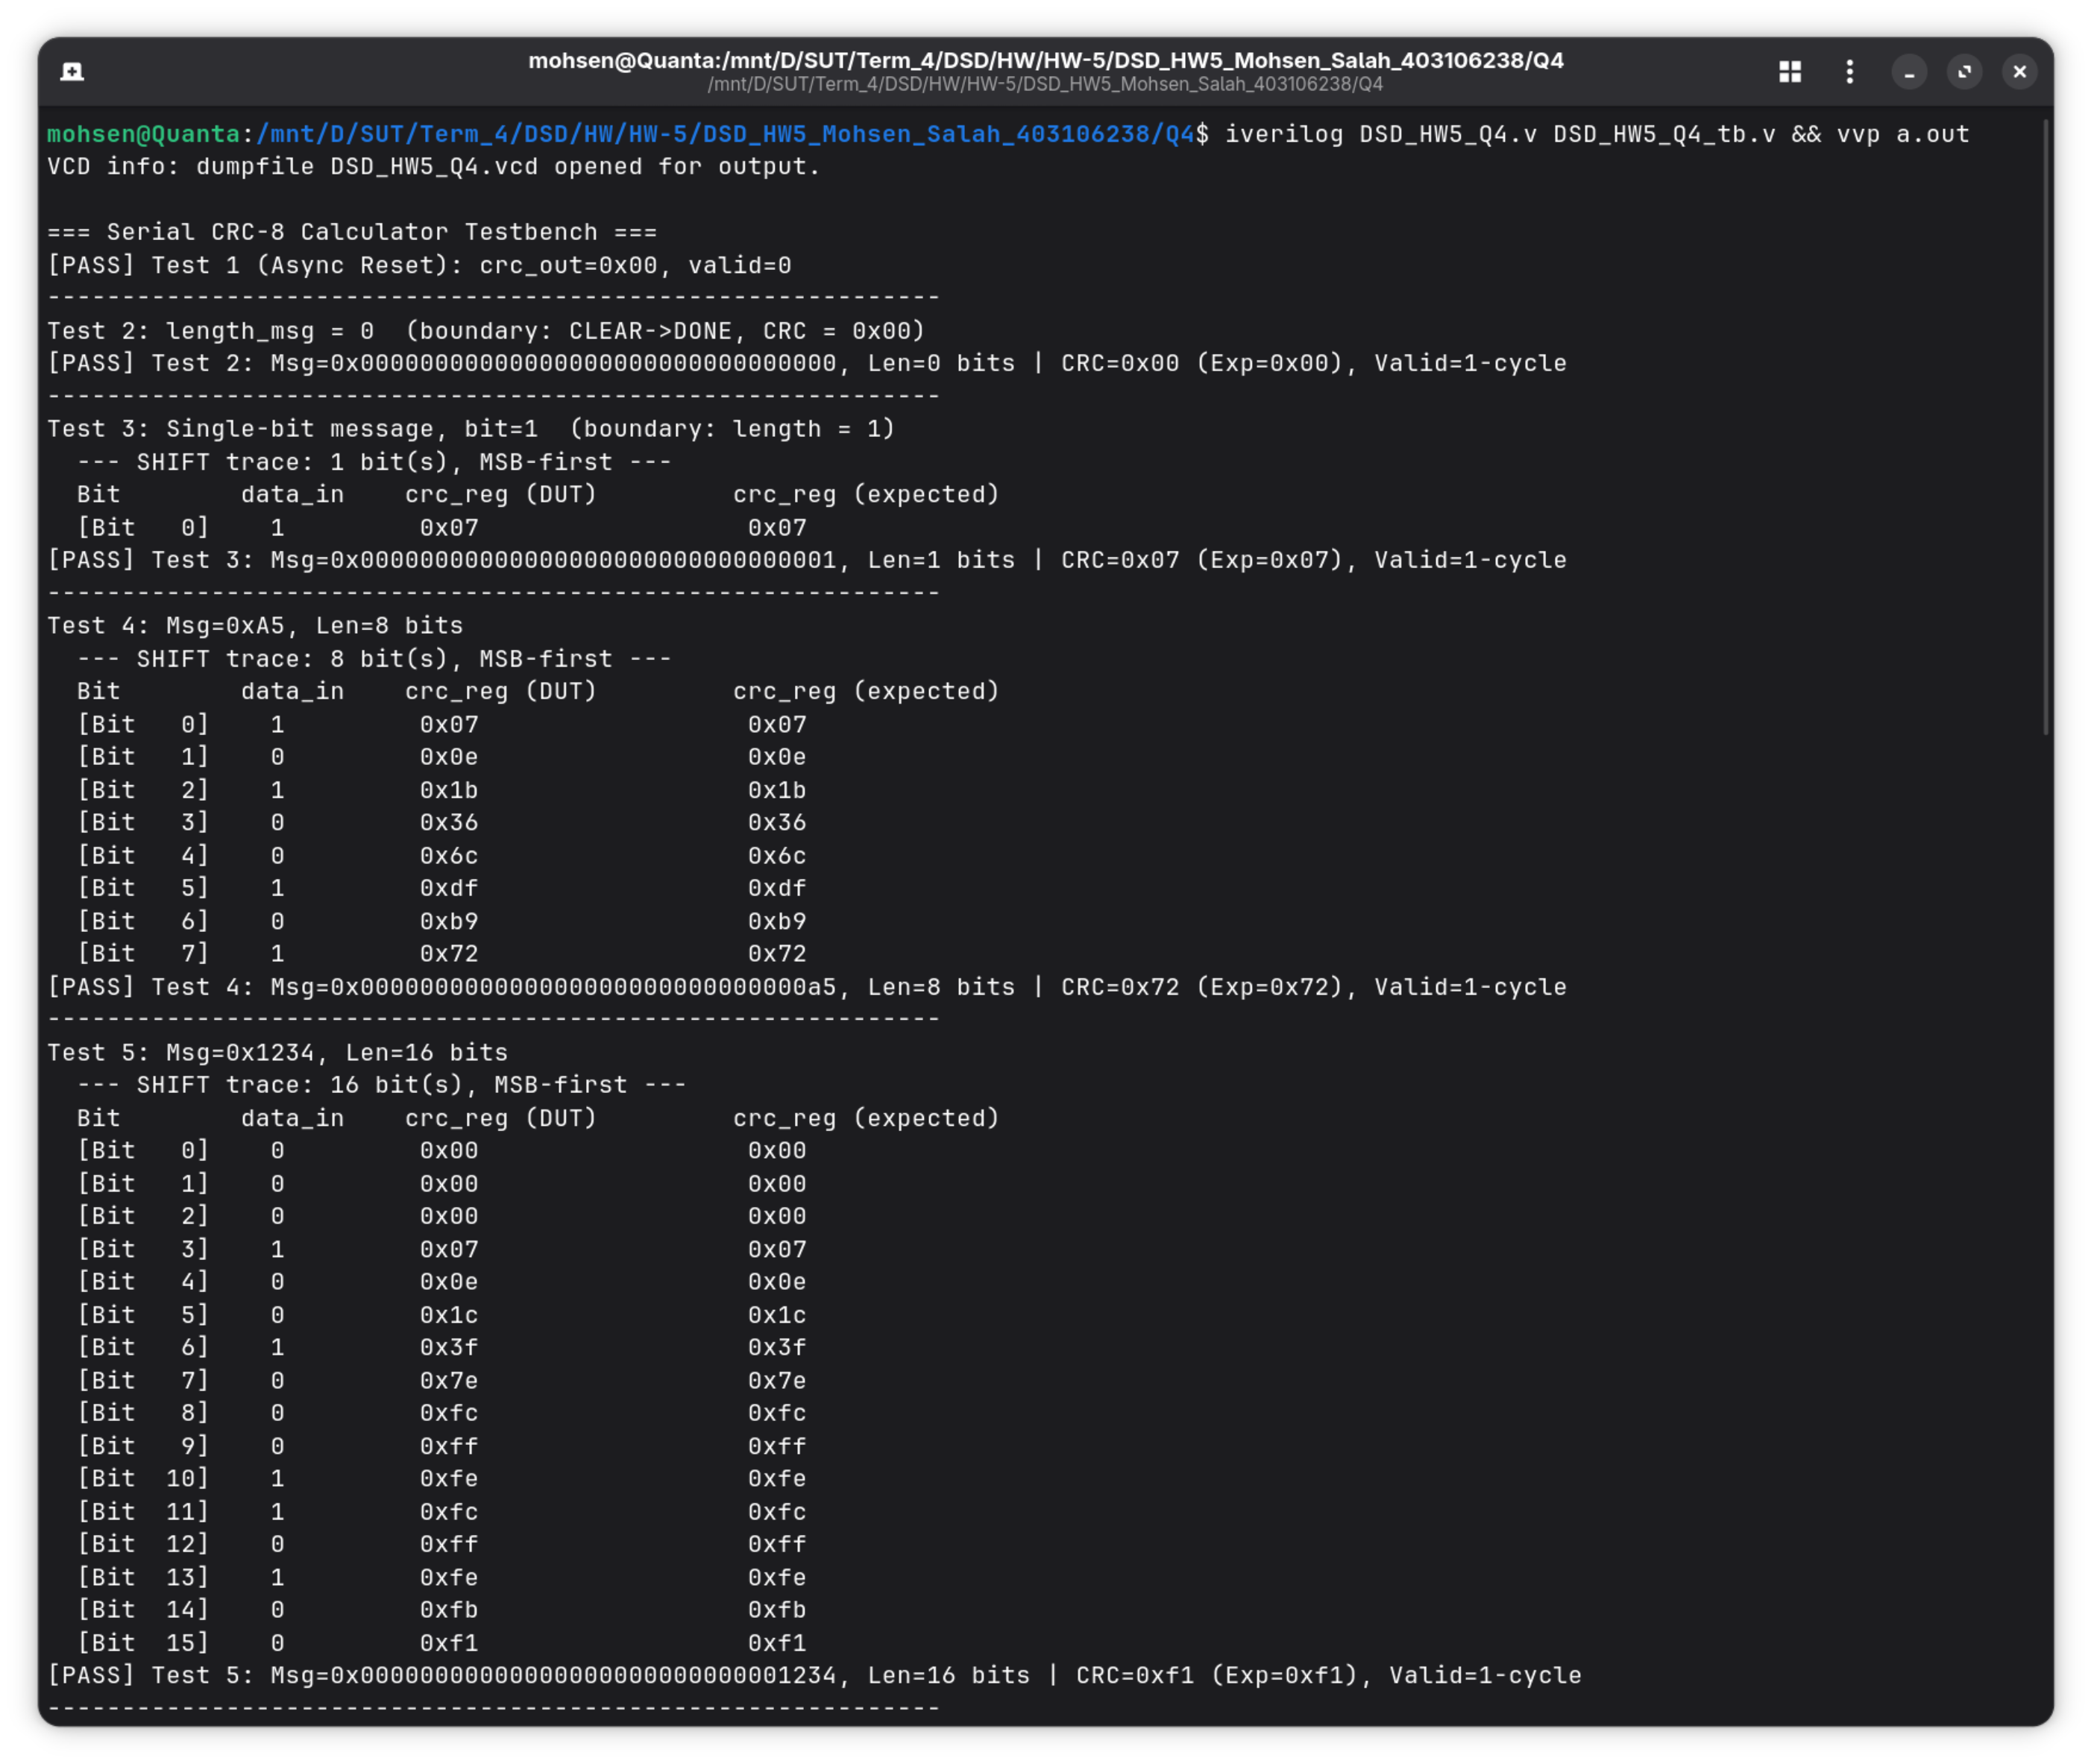
\includegraphics[width=0.9\textwidth]{assets/terminal_1.png}
    \caption{خروجی شبیه‌سازی در ترمینال}
\end{figure}

\begin{figure}[H]
    \centering
    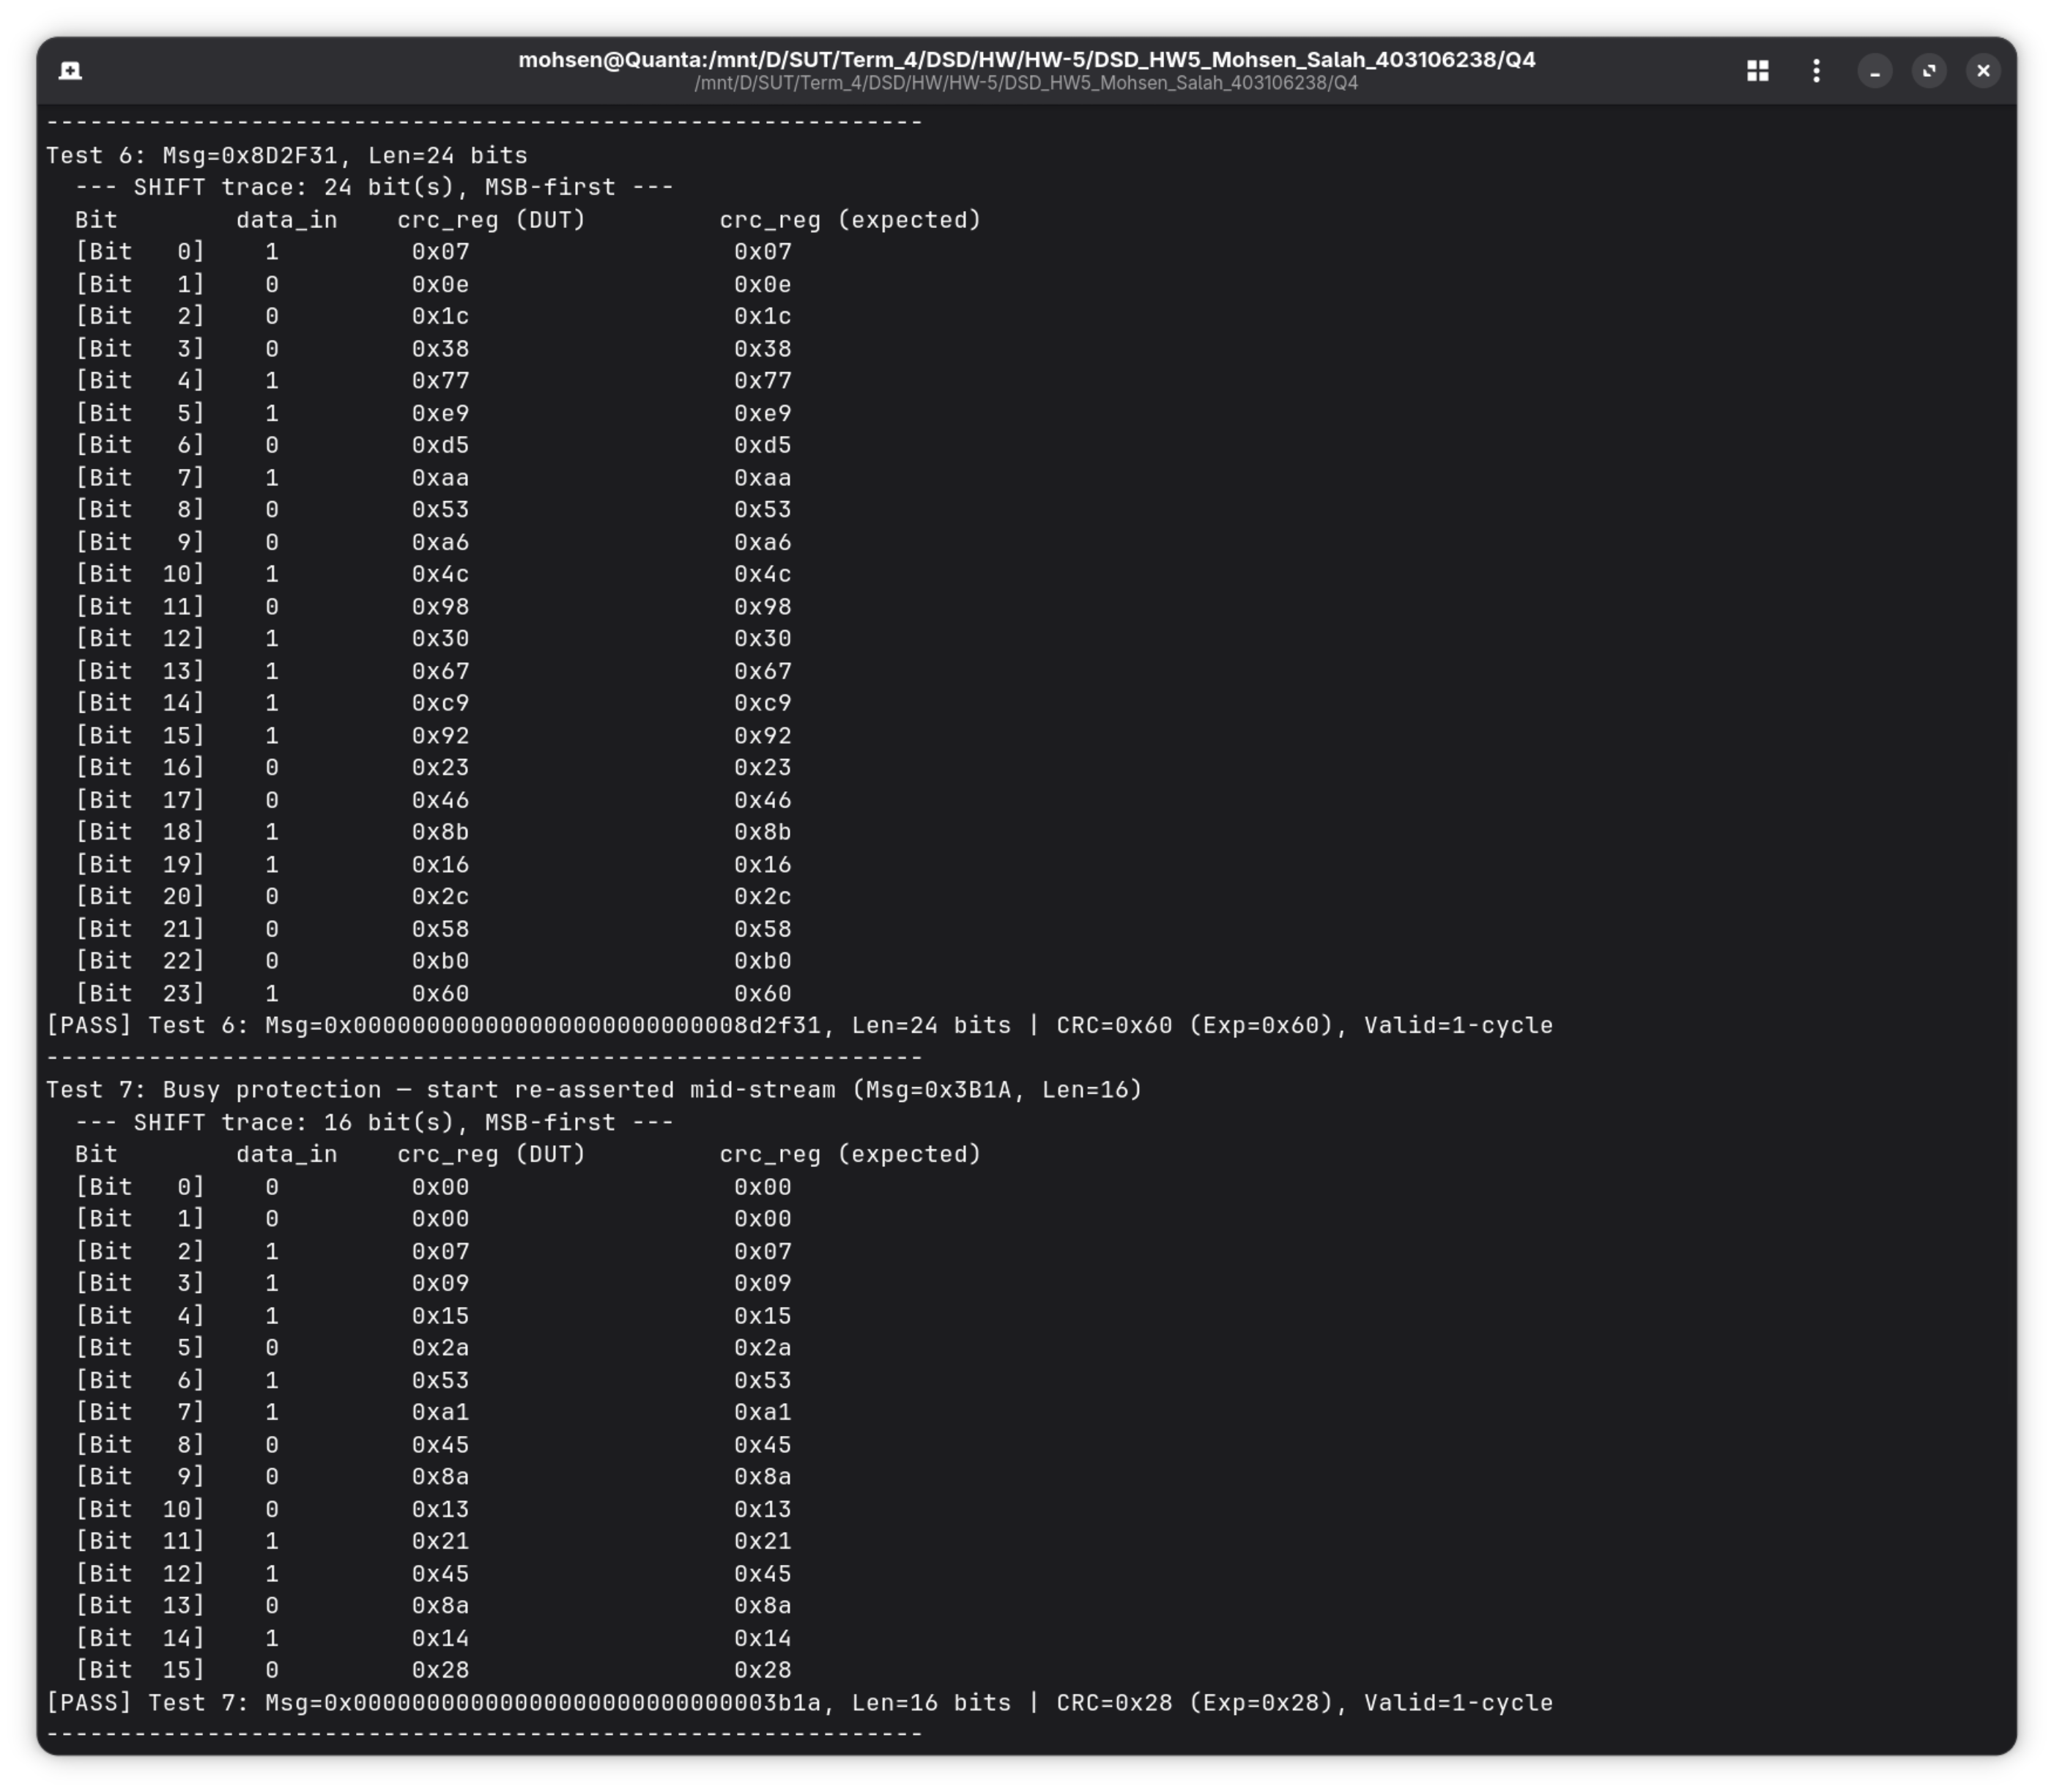
\includegraphics[width=0.9\textwidth]{assets/terminal_2.png}
    \caption{خروجی شبیه‌سازی در ترمینال (ادامه)}
\end{figure}

\begin{figure}[H]
    \centering
    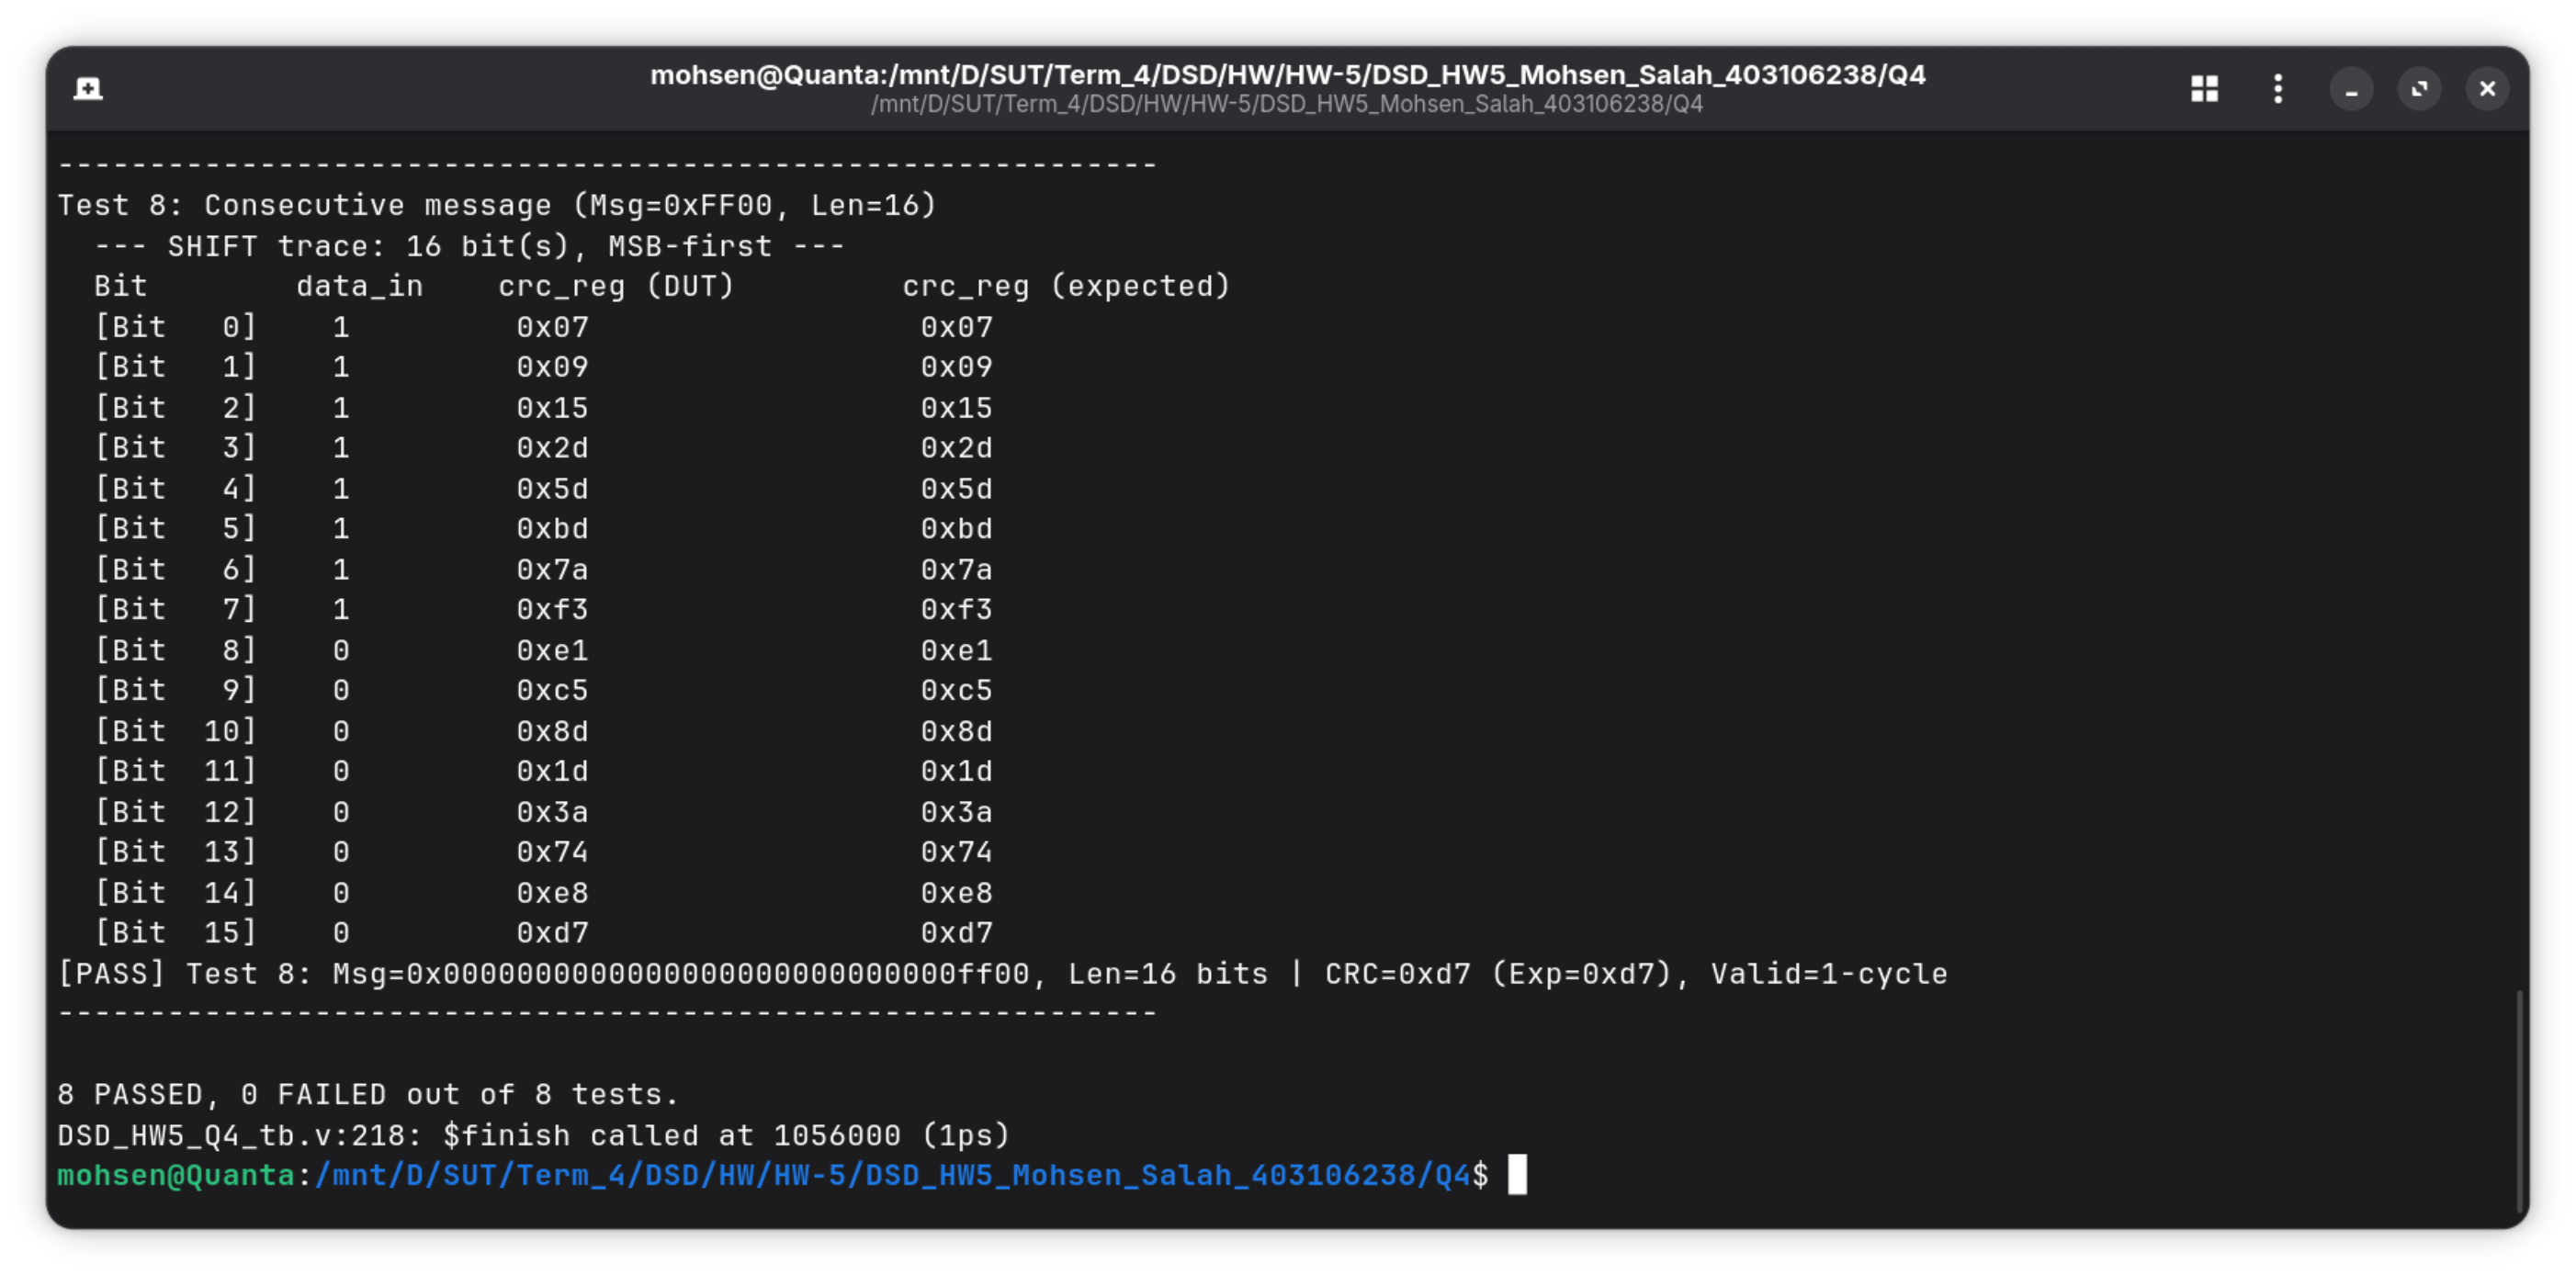
\includegraphics[width=0.9\textwidth]{assets/terminal_3.png}
    \caption{خروجی شبیه‌سازی در ترمینال (ادامه)}
\end{figure}

همان‌طور که مشاهده می‌شود، تمام ۸ تست با نتیجه \lr{PASS} اجرا شده‌اند.
در \lr{SHIFT trace} هر تست، مقدار \code{crc\_reg} در هر سیکل برابر مقدار
مورد انتظار مدل مرجع است که صحت سیم‌کشی چندجمله‌ای را تأیید می‌کند.

\begin{figure}[H]
    \centering
    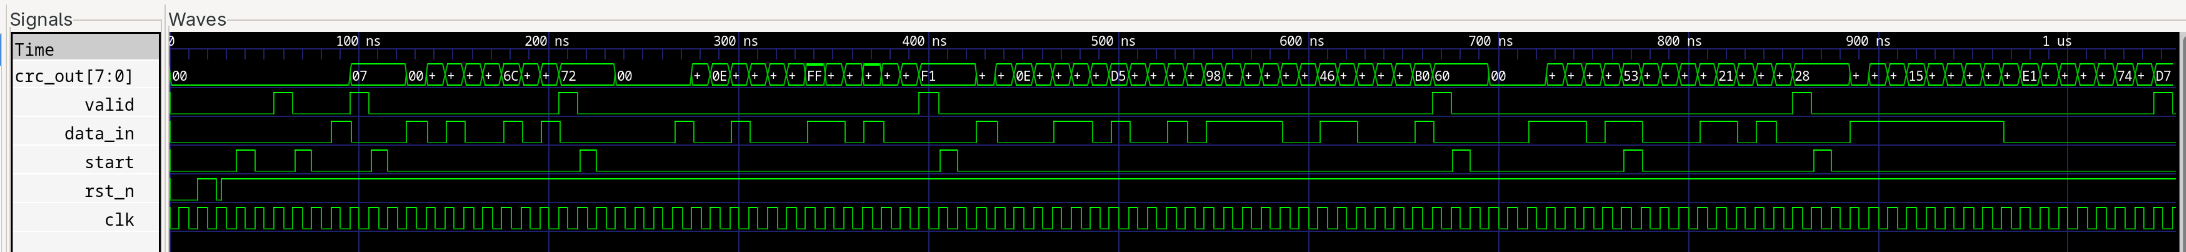
\includegraphics[width=1.0\textwidth]{assets/gtkwave.png}
    \caption{شکل‌موج سیگنال‌ها در \lr{GTKWave}}
\end{figure}

همان‌طور که مشاهده می‌شود، در هر اجرا \code{valid} دقیقاً یک سیکل فعال
می‌شود، \code{out\_crc} در همان سیکل مقدار صحیح را نشان می‌دهد، و سیستم
در سیکل بعد به \lr{IDLE} بازمی‌گردد. همچنین در تست ریست، پایین رفتن
\code{n\_rst} بلافاصله و خارج از لبه کلاک، \code{crc\_out} را صفر می‌کند.